\chapter{Modellazione Del Sistema}

\begin{definizione}[Sistema Distribuito]
Un \textit{sistema distribuito} è un insieme \textbf{entità} (dette anche \textbf{nodi}, \textbf{agenti}) che eseguono un algoritmo cooperando tra loro, comunicando e coordinandosi per raggiungere un obiettivo comune. Ogni nodo ha una propria memoria locale e può comunicare con altri nodi attraverso un canale di comunicazione. Internamente, ciascun nodo possiede un clock locale, che scandisce il tempo per le comunicazioni e le operazioni. I vari clock dei nodi non sono necessariamente sincronizzati tra loro, e possono procedere a velocità diverse. Inoltre, i nodi possono subire guasti, come crash o malfunzionamenti, che possono influenzare il comportamento del sistema.
\end{definizione}

Tale ambiente distribuito viene modellato mediante grafo $G = (V, E)$, dove $V$ ($|V| = n$) è l'insieme dei vertici (nodi) e $E$ ($|E| = m$) è l'insieme degli archi (interconnessioni). In particolar modo, data una
rete costituita da agenti e interconnessioni tra di essi, il grafo sottostante ha un vertice per
ciascun agente del sistema e un arco tra due nodi per ogni interconnessione tra i
corrispettivi agenti.

\section{Definizioni Elementari}

\begin{definizione}[Entità]
Un'ambiente distribuito è costituito da un insieme $\mathcal{E}$ di entità. Ogni nodo $x \in \mathcal{E}$ della rete, ha delle capacità computazionali, le quali sono definite come un insieme di operazioni possibili, tra le quali
\begin{itemize}
    \item \textbf{Comunicazione}: capacità di inviare e ricevere messaggi ad altri nodi della rete.
    \item \textbf{Local storage \& processing}: capacità di memorizzare e elaborare informazioni localmente.
    \item \textbf{Clock}: capacità di tenere traccia del tempo, impostando un clock locale che scandisce il tempo per le comunicazioni e le operazioni. I vari clock dei nodi non sono necessariamente sincronizzati tra loro, e possono procedere a velocità diverse.
    \item \textbf{Modificare registri locali}: capacità di modificare i propri \textbf{registri locali}, che rappresentano lo \text{stato interno del nodo}.
\end{itemize}
\end{definizione}

\begin{definizione}[Stato]
Definamo $\Sigma$ come l'insieme di tutti gli stati che può assumere un nodo $x \in \mathcal{E}$. L'insieme degli stati è definito a priori e deve essere un insieme finito. Ad esempio, 
\[
\Sigma = \{\text{idle}, \text{computing}, \text{waiting}, \dots\}
\]

È importante notare che ad ogni istante di tempo $t$, un nodo $x$ si trova in uno stato specifico $s \in \Sigma$. Lo stato di un nodo può cambiare nel tempo a seguito di operazioni computazionali o comunicazioni con altri nodi. Non esistono stati intermedi o transitori: un nodo è sempre in uno stato ben definito, e il passaggio da uno stato all'altro avviene in modo discreto, senza stati intermedi.
\end{definizione}

\begin{definizione}[Evento]
In un ambiente distribuito, il comportamento di ogni entità $x \in \mathcal{E}$ è \textbf{reattivo}, ovvero è indotto a
seguito del verificarsi di \textbf{eventi}. In assenza di stimoli, un'entità rimane inerte.

In generale, gli eventi possono essere di vario tipo, come ad esempio:
\begin{itemize}
    \item \textbf{Ricezione di un messaggio}: quando un nodo riceve un messaggio da un altro nodo, questo evento può indurre il nodo a cambiare stato o a eseguire determinate operazioni. 
    \item \textbf{Tick del clock}: quando il clock locale di un nodo raggiunge un certo valore, questo evento può indurre il nodo a eseguire determinate operazioni o a cambiare stato.
    \item \textbf{Evento spontaneo}: un nodo può essere indotto a eseguire determinate operazioni o a cambiare stato in modo spontaneo.
\end{itemize}
\end{definizione}

\begin{definizione}[Azione]
Un' \textbf{azione} è una trasformazione che può essere eseguita da un nodo $x \in \mathcal{E}$ in risposta a un evento. Ogni azione modifica lo stato di un nodo o invia un messaggio ad un altro nodo. Formalmente, è una funzione \textbf{deterministica} che, fissato un istante di tempo $t$, mappa tutte le coppie (stato, evento) in un'azione specifica.

\[
f: \Sigma \times \hat{E} \rightarrow \mathcal{A}
\]

dove $\mathcal{A}$ è l'insieme di tutte le \textbf{sequenze di task} che possono essere eseguite, e $\hat{E}$ è l'insieme di tutti gli eventi che possono verificarsi in un ambiente distribuito.

In generale, un'azione può consistere in:
\begin{itemize}
    \item \textbf{computare} un algoritmo;
    \item \textbf{inviare} messaggi ad altri nodi;
    \item \textbf{modificare} lo stato interno del nodo.
\end{itemize}

In questo modello, ogni azione è \textbf{atomica} e \textbf{finita}:
\begin{itemize}
    \item \textbf{Atomica}: una volta avviata, un'azione non può essere interrotta;
    \item \textbf{Finita}: un'azione termina sempre in tempo finito.
\end{itemize}

Si osserva che un'entità in un certo stato potrebbe non reagire a un evento: in questo caso si assume che l'entità abbia eseguito l'azione \textit{nil} (azione nulla).
\end{definizione}

\begin{definizione}[Comportamento di un'entità]
    Le associazioni (stato, evento) $\rightarrow$ azione, per ogni nodo $x \in \mathcal{E}$, sono dette \textbf{regole}. Definiamo il \textbf{comportamento} di un'entità $x$ come l'insieme di tutte le regole che governano le azioni che il nodo esegue in risposta a eventi specifici, a seconda dello stato in cui si trova. Diremo che il comportamento di un'entità è 
    \begin{itemize}
        \item \textbf{deterministico} se, per ogni coppia (stato, evento), esiste una regola che associa un'unica azione,
        \item \textbf{completo} se per ogni coppia (stato, evento) esiste almeno una regola che associa un'azione.
    \end{itemize}

    Il \textbf{comportamento} di un nodo $x \in \mathcal{E}$ è descrivibile mediante l'insieme $B(x)$ che deve essere \textbf{non-ambiguo} e \textbf{completo}, ossia:
    \[
    \forall (s, e) \in \Sigma \times \hat{E}, \exists!\ a \in \mathcal{A} : f(s, e) = a
    \]
\end{definizione}

\begin{definizione}[Comportamento del Protocollo]
    Definiamo il \textbf{comportamento del protocollo} come l'insieme di tutti i comportamenti dei nodi che partecipano al sistema distribuito. Formalemente è descritto come:
    \[
    B(\mathcal{E}) = \{B(x) : x \in \mathcal{E}\}
    \]

    Un sistema si dice \textbf{simmetrico (o omogeneo)} se tutti i nodi condividono lo stesso comportamento, ovvero:
    \[
    B(x) \equiv B(y)\quad \forall\ x, y \in \mathcal{E}
    \]

    Si nota che un sistema simmetrico è caratterizzato da un protocollo unico che viene eseguito da tutti i nodi. Questo significa che durante l'esecuzione i nodi posso effettuare azioni diverse ma il protocollo deve essere lo stesso. In un sistema asimmetrico (o eterogeneo), l'azione del singolo nodo dipende dalla sua etichetta.

    In un sistema \textbf{asimmetrico (o eterogeneo)}, il comportamento del singolo nodo dipende dalla sua identificazione o dal suo ruolo. Tuttavia, qualsiasi sistema asimmetrico può essere trasformato in uno simmetrico riscrivendo l'insieme di regole in modo che l'azione eseguita dipenda dalla tipologia del nodo.

    \textbf{Esempio}: Consideriamo un sistema con due tipologie di entità: server e client, ognuna con un insieme di regole differenti. È possibile unificare i comportamenti creando un nuovo insieme di regole simmetrico in cui ogni nodo esegue la stessa logica, ma l'azione concreta varia in base al ruolo dell'entità. In questo modo, il protocollo rimane unico e simmetrico per tutti i nodi.
\end{definizione}

\begin{definizione}[Comunicazione]
Le entità in un sistema distribuito interagiscono attraverso lo \textbf{scambio di messagl'insieme dei nodi con cui $x$ può comunicare direttamente, ossia:gi (message passing)}. Un messaggio è una \textbf{sequenza finita di bit} che transita su canali di comunicazione tra nodi. La topologia di comunicazione è rappresentata da un grafo diretto $G = (V, E)$ ($V = \mathcal{E}$), dove un arco $(x, y) \in E$ indica che il nodo $x$ può inviare messaggi al nodo $y$. Non tutti i nodi possono comunicare direttamente: la capacità di comunicazione tra due nodi è determinata dalla struttura della rete sottostante.

Si osserva che i nodi \textit{non hanno una visione globale} del sistema (ossia non conoscono la tologia del grafo della rete), ma solo una \textbf{visione locale}. Formalemente, $\forall x \in V$, possiamo definire gli insieme:
\begin{itemize}
    \item $N_{\text{out}}(x) = \{y \in V : (x, y) \in E\} \subset V$, l'insieme dei nodi a cui $x$ può inviare messaggi (\textit{archi uscenti});
    \item $N_{\text{in}}(x) = \{y \in V : (y, x) \in E\}  \subset V$, l'insieme dei nodi da cui $x$ può ricevere messaggi (\textit{archi entranti}).
\end{itemize}

Dunque, definiamo il \textbf{vicinato} di un nodo $x$ come 
\[
N(x) = N_{\text{out}}(x) \cup N_{\text{in}}(x)
\]
\end{definizione}

\begin{definizione}[Tempo di Terminazione]
Un protocollo si dice \textbf{terminante} se, a partire da qualsiasi configurazione iniziale, raggiunge una configurazione finale in un tempo finito. Formalmente, esiste un tempo finito $t$ tale che, per ogni nodo $x \in V$, il nodo raggiune uno stato \textit{quiescente} (ossia, uno stato in cui non esegue più azioni) entro $t$.
\end{definizione}

\begin{definizione}[Tempo di Completamento]
Un protocollo si dice \textbf{completante} se, a partire da qualsiasi configurazione iniziale, raggiunge una configurazione finale \textbf{accettabile} in un tempo finito. In altre parole, esiste un istante di tempo finito $t$, per cui il task è risolto, ossia, ogni nodo $x \in V$ si trova in uno stato accettabile entro $t$.
\end{definizione}

In generale, un protocollo terminante non è necessariamente completante, e viceversa.

\section{Assiomi e Restrizioni}

La definzione di sistema distribuito è accompagnata da 2 \textit{assiomi fondamentali}. Qualsisi assunzione aggiuntiva che si vuole fare su un sistema distribuito sarà chiamata \textit{restrizione}

\subsection{Assiomi}

\begin{description}
    \item[Finite Transmission Delays] In assenza di perdite di messaggi, si assume che il tempo di trasmissione di un messaggio tra due nodi sia finito. Ciò implica che, se un nodo invia un messaggio a un altro nodo, il messaggio arriverà entro un tempo finito, anche se questo tempo può essere arbitrariamente lungo, di conseguenza, il sistema non è a conoscenza di questo tempo di trasmissione.
    
    Formalmente, $\forall$ messaggio $m$ inviato da un nodo $x$ a un nodo $y$, esiste un tempo finito $\tau_{xy} \in \mathbb{R}^+$ tale che $m$ arriva a $y$ entro $\tau_{xy}$.
    \item[Local Orientation] Questo assioma stabilisce che ogni nodo distingue localmente i suoi vicini, ossia, distingue tra gli archi entranti e quelli uscenti. Un'entità è sempre in grado di inviare un messaggio solamente ad uno specifico e singolo vecino uscente. Di conseguenza, è in grado di distinguere quale dei suoi vicini gli ha inviato un messaggio. Formalemten, ogni nodo $x$ ha una funzione locale iniettiva di orientamento, che assegna un'etichetta univoca a ciascun arco:
    \[ 
    \lambda_x: E_x \rightarrow L
    \]
    dove $E_x = \{ (x, y) \in E \}$ è l'insieme degli archi incidenti su $x$ e $L$ è un insieme di etichette.

    Possiamo quindi discutere di grafi etichettati $(G, \lambda)$ ($\lambda = \{\lambda_x: x \in V\}$), dove ogni arco (\textbf{non nodo}) $(x, y)$ ha un'etichetta \textbf{locale} $\lambda_x(x, y)$ che identifica univocamente il vicino $y$ per il nodo $x$. Allo stesso modo, l'arco $(y, x)$ avrà un'etichetta $\lambda_y(y, x)$ che identifica $x$ per il nodo $y$.

    \begin{figure}[ht!]
        \centering
        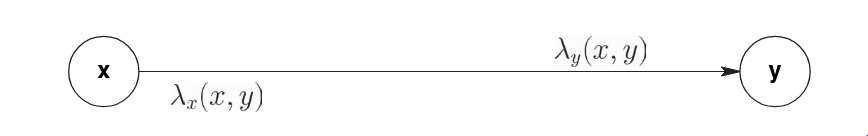
\includegraphics[width=0.8\linewidth]{images/orientation.png}
        \caption{Ciascun arco ha due etichette.}
        \label{fig:orientation}
    \end{figure}

    In generale, $\lambda_x(x, y) \neq \lambda_y(x, y)$.
\end{description}

\subsection{Resitrizioni}
Spesso i protocolli vengono definiti e studiati assumendo ulteriori restrizioni. Naturalmente
un protocollo definito sotto un gran numero di restrizioni è generalmente debole, nel senso
che, rimuovendo alcune di queste restrizioni, il protocollo potrebbe non risolvere il problema
preso in analisi. Un protocollo definito su un sistema con poche restrizioni invece risulta più
generale, e dunque più forte.

Si elencano alcune tipologie di restrizioni.

\begin{description}
    \item[Message Ordering] Si assume che i messaggi inviati da un nodo $x$ a un nodo $y$ arrivino in ordine FIFO (First In First Out) (\textbf{FIFO queue}). Ciò significa che se $x$ invia due messaggi $m_1$ e $m_2$ a $y$, con $m_1$ inviato prima di $m_2$, allora $y$ riceverà $m_1$ prima di $m_2$. Questa restrizione semplifica la progettazione dei protocolli, poiché garantisce un ordine prevedibile dei messaggi tra coppie di nodi.
    \item[Bidirectional Links] Si assume che le connessioni tra nodi sia \textit{bidirezionale}, ossia, $\forall x
    , y \in \mathcal{E}$, se $(x, y) \in E$, allora anche $(y, x) \in E$ e inoltre $\lambda_x(x, y) = \lambda_y(y, x)$. Questa restrizione implica che se un nodo $x$ può inviare messaggi a un nodo $y$, allora $y$ può anche inviare messaggi a $x$, e che entrambi i nodi condividono la stessa etichetta per identificare la connessione tra di loro. Questa restrizione semplifica la progettazione dei protocolli, poiché garantisce una comunicazione simmetrica tra i nodi. Formalmente, 
    \[
        \forall x \in V,\ N_{\text{out}}(x) = N_{\text{in}}(x) = N(x) \quad \text{e} \quad \lambda_x(x, y) = \lambda_y(y, x) \quad \forall y \in N_{\text{out}}(x)
    \]
    \begin{figure}[ht!]
        \centering
        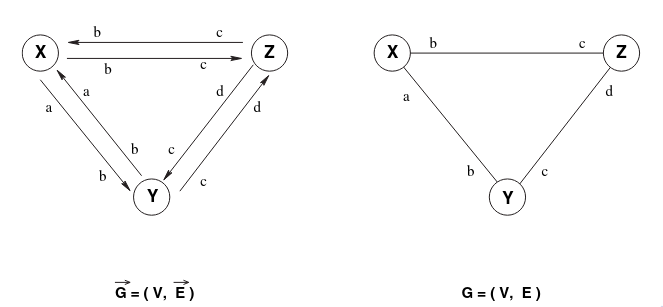
\includegraphics[width=0.8\linewidth]{images/bidirectional.png}
        \caption{In una rete con archi bidirezionali, consideriamo il corrispondente grafo semplificato non diretto.}
        \label{fig:bidirectional}
    \end{figure}
    \item[Reliability Restrictions] Ci chiediamo: cosa succede al messaggio durante il traggitto? Possiamo fare delle assunzioni sulla disponibilità dei canali di comunicazione. 
    \begin{itemize}
        \item \textbf{Guaranteed Delivery}: Ogni messaggio che viene inviato viene \textbf{ricevuto correttamente}, cioè non ci sono corruzioni di messaggi. Sotto questa restrizione, i protocolli non devono tenere conto di omissioni o corruzioni dei messaggi durante la trasmissione.
        \item \textbf{Partial Reliability}: Non si verificano guasti (ad esempio crash dei nodi, perdità di messaggi) dall'istante in cui si inizia ad osservare il sistema. Si osserva che, negli istanti precendenti all'inzio dell'osservazione, il sistema potrebbe aver subito guasti.
        \item \textbf{Total Reliability}: Non sono mai avvenuti fallimenti e mai avverranno in futuro.
    \end{itemize}
    \item[Topological Restrictions] In genere consistono in assunzioni sulla topologia del grafo della rete. Ad esempio assumere che il grafo sia \textbf{connesso/fortemente connesso}.
    \item[Knowledge Restrictions] Assumiamo quali sono le informazioni che ogni nodo conosce riguardo la rete. Ad esempio in numero di nodi ($|V| = n$), oppure il numero di archi ($|E| = m$), il diametro della rete, l'etichettamento universale, etc... .
    \item[Time Restrictions] Eccetto il tempo di trasmissione finito, il modello generale non fa assunzioni su tale quantità.
    Due possibili restrizioni riguardo i tempi di comunicazione sono le seguenti:
    \begin{itemize}
        \item \textbf{Bounded Communication Delay:} Esiste una costante $\Delta$ tale che, in assenza di guasti, il delay dei messaggi è al più $\Delta$, in altre parole se un nodo $x$ invia un messaggio $m$ ad un nodo $y$, $m$ arriverà ad $y$ in al più $\Delta$ istanti di tempo.
        \item \textbf{Syncronized Clock:} Tutti i nodi condividono un clock globale sincronizzato, ossia, $\forall x, y \in \mathcal{E}$, $clock_x(t) = clock_y(t)$ per ogni istante di tempo $t$. Questa restrizione semplifica la progettazione dei protocolli, poiché consente ai nodi di coordinare le loro azioni basandosi su un riferimento temporale comune.
    \end{itemize}
    \item[Cost \& Complexity Measures] In generale in un sistema distribuito non ha senso parlare di complessità temporale, poiché non è detto che i nodi condividano un clock globale. Per parlare di complessità temporale è necessario assumere la \textit{Syncronized Clock} e la \textit{Bounded Communication Delay}. 
    
    Parleremo spesso di \textbf{messagge complexity}, ovvero una misura che tiene conto del numero di messaggi scambiati durante l'esecuzione di un protocollo. Parleremo quindi di numero di bit scambiati, o di numero di messaggi scambiati.
\end{description}
